\documentclass{beamer}%
\usepackage[T1]{fontenc}%
\usepackage[utf8]{inputenc}%
\usepackage{lmodern}%
\usepackage{textcomp}%
\usepackage{lastpage}%
%
\title{Sample Beamer Presentation}%
\author{Your Name}%
\date{\today}%
%
\begin{document}%
\normalsize%
\frame{\titlepage}%

\begin{frame}%
\frametitle{Introduction}%
This is the first slide. Welcome to the presentation!%
\end{frame}%

\begin{frame}%
\frametitle{Contents}%
This talk will two main parts:
\begin{itemize}%
\item Running a Linux VM on my mobile phone.
\item My pet project with NLP. 
\end{itemize}%
\end{frame}%

\section{Linux on my phone}

\begin{frame}{Title of the Slide}

\begin{columns}

% Left column: bullet points
\begin{column}{0.5\textwidth}
\begin{itemize}
\item First point
\item Second point
\item Third point
\item Fourth point
\end{itemize}
\end{column}

% Right column: figure
\begin{column}{0.5\textwidth}
\centering

\includegraphics[width=\linewidth]{cake.jpg} % Replace with your image file
\end{column}
\end{columns}
\end{frame}

\begin{frame}%
\frametitle{Main Points}%
\begin{itemize}%
\item Point 1%
\item Point 2%
\item Point 3%
\end{itemize}%
\end{frame}%

\begin{frame}{Delicious Cake}
    \begin{center}
            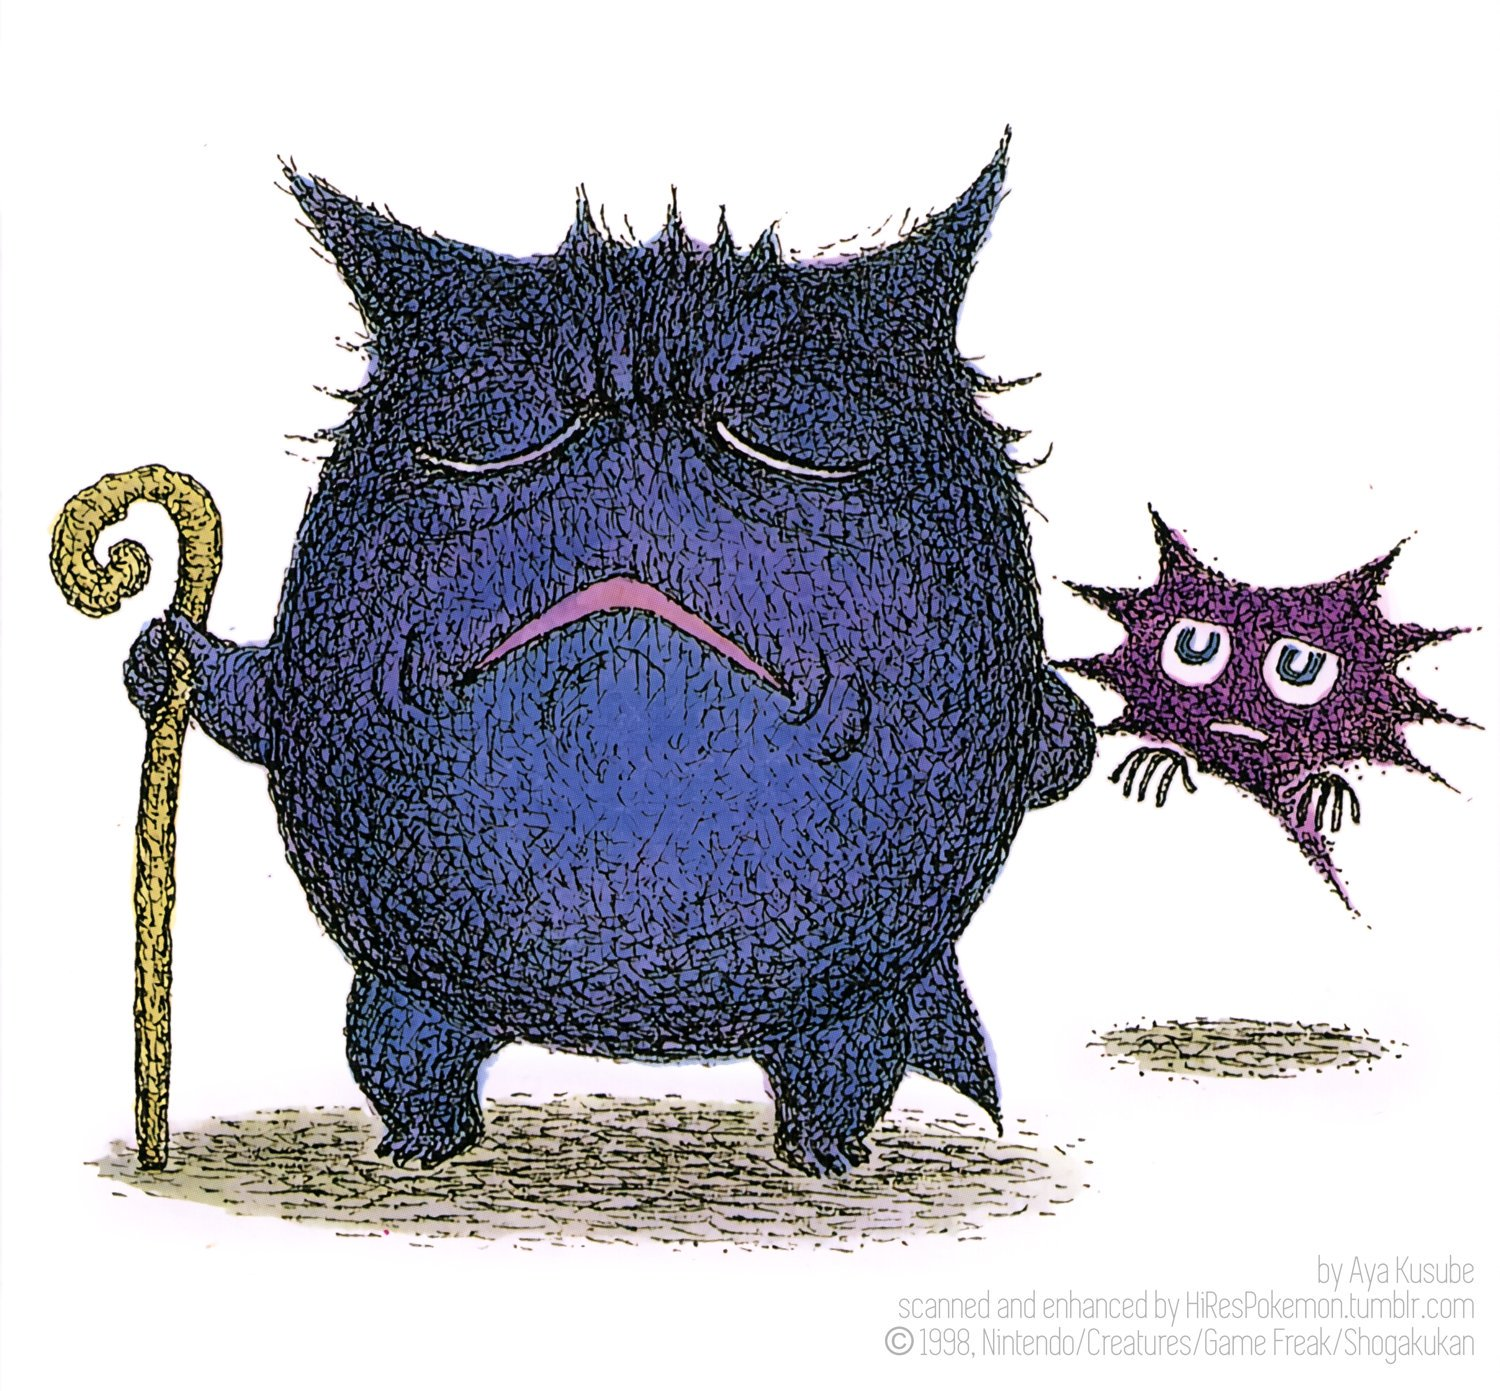
\includegraphics[width=0.8\linewidth]{gengar.jpeg}
    \end{center}
\end{frame}

\begin{frame}%
\frametitle{Conclusion}%
Thank you for your attention!%
\end{frame}%
\end{document}
